\documentclass{standalone}
%\documentclass[a4paper,aps,prl,onecolumn]{revtex4}

\usepackage{graphicx} %[dvips]
\usepackage[usenames,dvipsnames]{xcolor}

\usepackage{tikz}
\usepackage{amsmath}
\usepackage{amssymb}
%\usepackage{natbib}
%\usepackage{color}
%\usepackage{float}
%\usepackage{epstopdf}
\usepackage[normalem]{ulem}
\usepackage{pgfplots,pgfplotstable}
\usepackage{hyperref}
\usepackage{soul}
\usepackage{comment}

\usetikzlibrary[shadings]
\usetikzlibrary{shapes}
\usetikzlibrary{snakes}

%% A text box with a white background and rounded edges
\newcommand*{\wbox}[1]{%
	\tikz[baseline=(X.base)] \node[rectangle, fill=white, rounded corners, inner sep=0.6mm] (X) {#1};%
}

\newcommand{\vett}[1]{\mathbf{#1}}
\newcommand {\Curl} {\mbox{\rm curl\,}}
\newcommand {\Skw} {\mbox{\rm skw\,}}
\newcommand {\Sym} {\mbox{\rm $\mathbb{S}$ym\,}}
\newcommand {\PSym} {\mbox{\rm P$\mathbb{S}$ym\,}}
\newcommand {\Lin} {\mbox{\rm $\mathbb{L}$in\,}}
\newcommand {\sym} {\mbox{\rm sym\,}}
\newcommand {\Div} {\mbox{\rm div\,}}
\newcommand {\tr} {\mbox{\rm tr\,}}
\newcommand {\sph} {\mbox{\rm sph\,}}
\newcommand {\sgn} {\mbox{\rm sgn\,}}
\newcommand{\minus}{\scalebox{0.6}[1.0]{$-$}}
\newenvironment{sistema}%
{\left\lbrace\begin{array}{@{}l@{}}}%
{\end{array}\right.}

\definecolor{IBM1}{HTML}{648fff}
\definecolor{IBM2}{HTML}{785ef0}
\definecolor{IBM3}{HTML}{dc267f}
\definecolor{IBM4}{HTML}{fe6100}
\definecolor{IBM5}{HTML}{ffb000}
\definecolor{IBM6}{RGB}{051,117,056}

\definecolor{Okabe1}{RGB}{000,158,115}
\definecolor{Okabe2}{RGB}{000,114,178}
\definecolor{Okabe3}{RGB}{086,180,233}
\definecolor{Okabe4}{RGB}{230,159,000}
\definecolor{Okabe5}{RGB}{213,094,000}
\definecolor{Okabe6}{RGB}{204,121,167}

\definecolor{b1}{HTML}{d73027}
\definecolor{b2}{HTML}{fc8d59}
\definecolor{b3}{HTML}{fee090}
\definecolor{b4}{HTML}{e0f3f8}
\definecolor{b5}{HTML}{91bfdb}
\definecolor{b6}{HTML}{4575b4}


\pgfplotsset{compat=newest}

\begin{document}





\begin{tikzpicture}
\label{Lp}
\begin{axis}[
	width=9cm,
	height=6cm,
	enlargelimits=false,
	title={$a.$},
	title style={yshift=-2ex, xshift=-33ex},
	tick pos=left,
	tick align=outside,
	axis line style={opacity=0},
	after end axis/.code={
		\draw ({rel axis cs:0,0}
		-|{axis cs:0,0}) % xmin (line starts here)
		-- ({rel axis cs:0,0}
		-|{axis cs:16,0}); % xmax (line stops here)
		\draw ({rel axis cs:0,0}
		|-{axis cs:0,0}) % ymin (line starts here)
		-- ({rel axis cs:0,0}
		|-{axis cs:0,15}); % ymax (line stops here)
	},
	grid=none,
	x label style={at={(axis description cs:0.5,-0.1375)},anchor=north},
	y label style={at={(axis description cs:-.075,.45)},rotate=0,anchor=south},
	xlabel style={xshift=-1.25cm},
	xlabel={$\delta$ (mm)},
	ylabel={$F$ (N)},
	legend style={at={(0.025,1)}, anchor=north west},
	xmin=-0.2,
	xmax=24,
	ymin=-0.2,
	ymax=15,
	ytick={0, 5, 10, 11.53, 15},
	yticklabels = {0, 5, 10, \textcolor{black}{$F_c$}, 15},
	y tick label style={
		/pgf/number format/.cd,
		fixed,
		fixed zerofill,
		precision=0,
		/tikz/.cd
	},
	xtick={0, 4, 8, 10.38, 12, 16},
	xticklabels = {0, 4, 8, \textcolor{black}{$\delta_c$}, 12, 16},
	x tick label style={
		/pgf/number format/.cd,
		fixed,
		fixed zerofill,
		precision=0,
		/tikz/.cd
	}
	]

]
	\addplot[color = Okabe2, ultra thick]  table[x index = 14, y index = 32, col sep=comma]{results_file.csv};
	\addplot[color = Okabe4, ultra thick]  table[x index = 2, y index = 20, col sep=comma]{results_file.csv};
	
	\addplot[color = Black!50, ultra thick]  table[x index = 37, y index = 38, col sep=comma]{results_file.csv};
	
	\node[anchor=south west,inner sep=0] at (16,9) {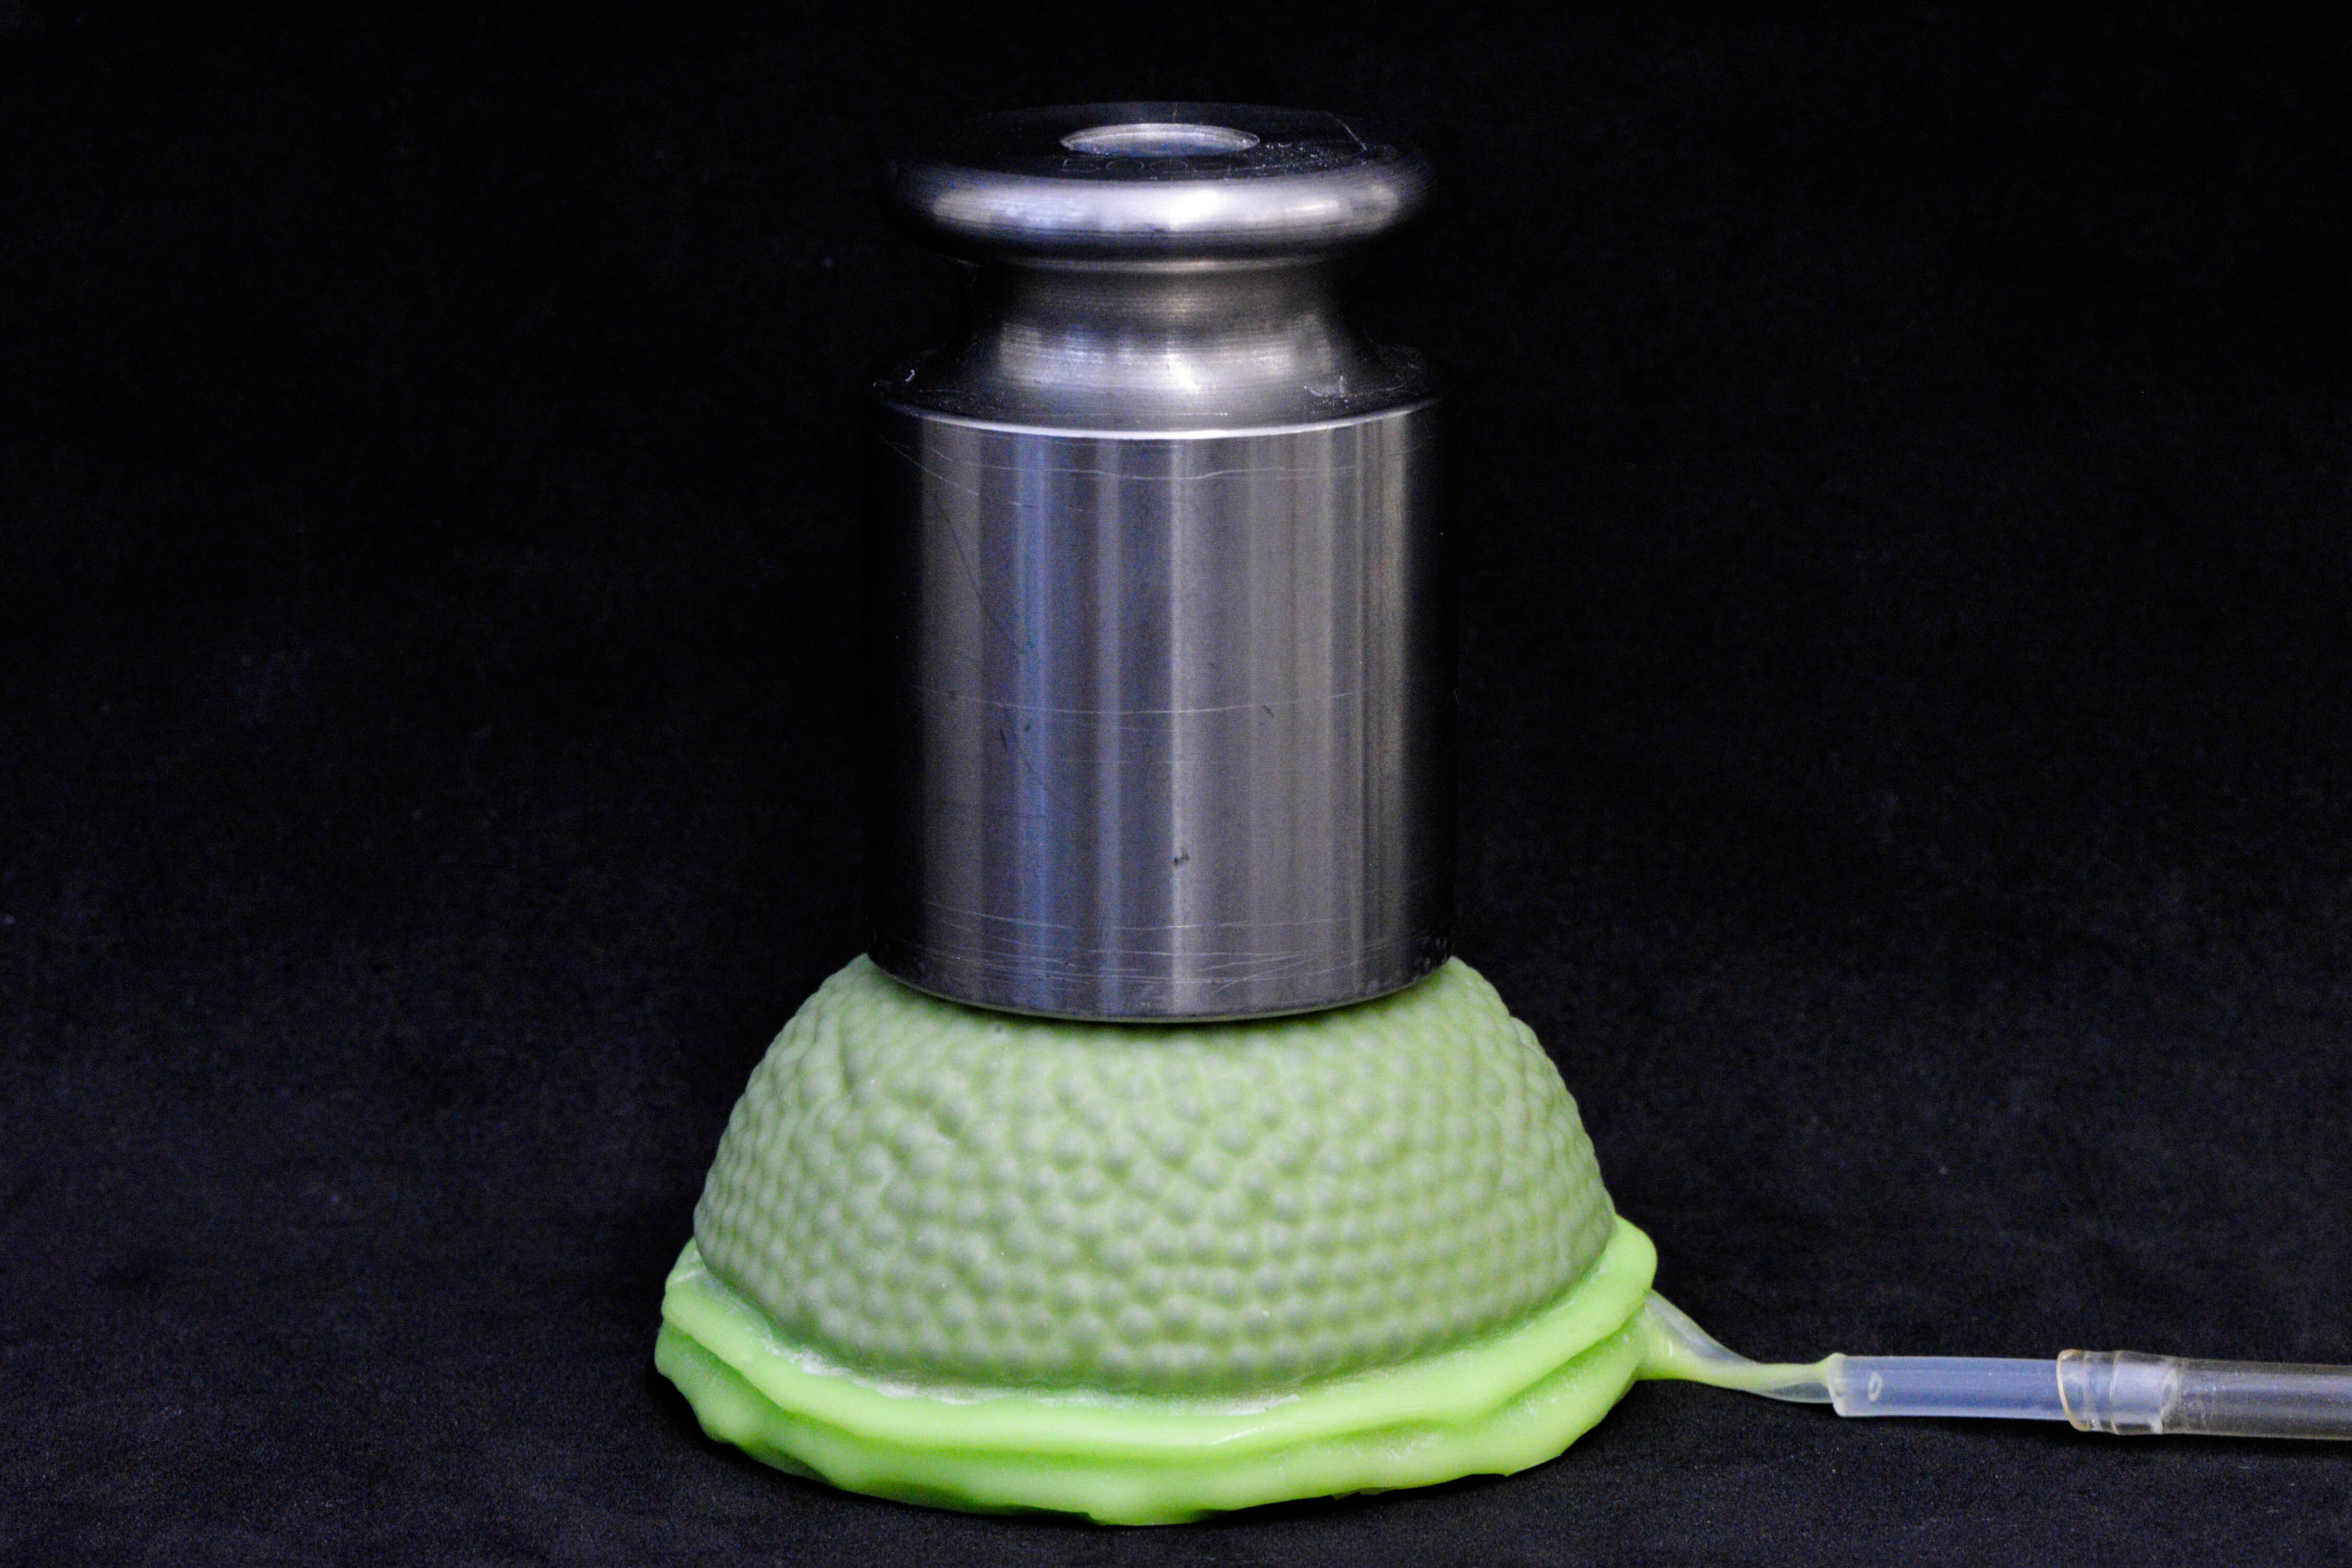
\includegraphics[height=1.5cm]{newShellHold-2}};
	\node[anchor=south west,inner sep=0] at (16,0.5) {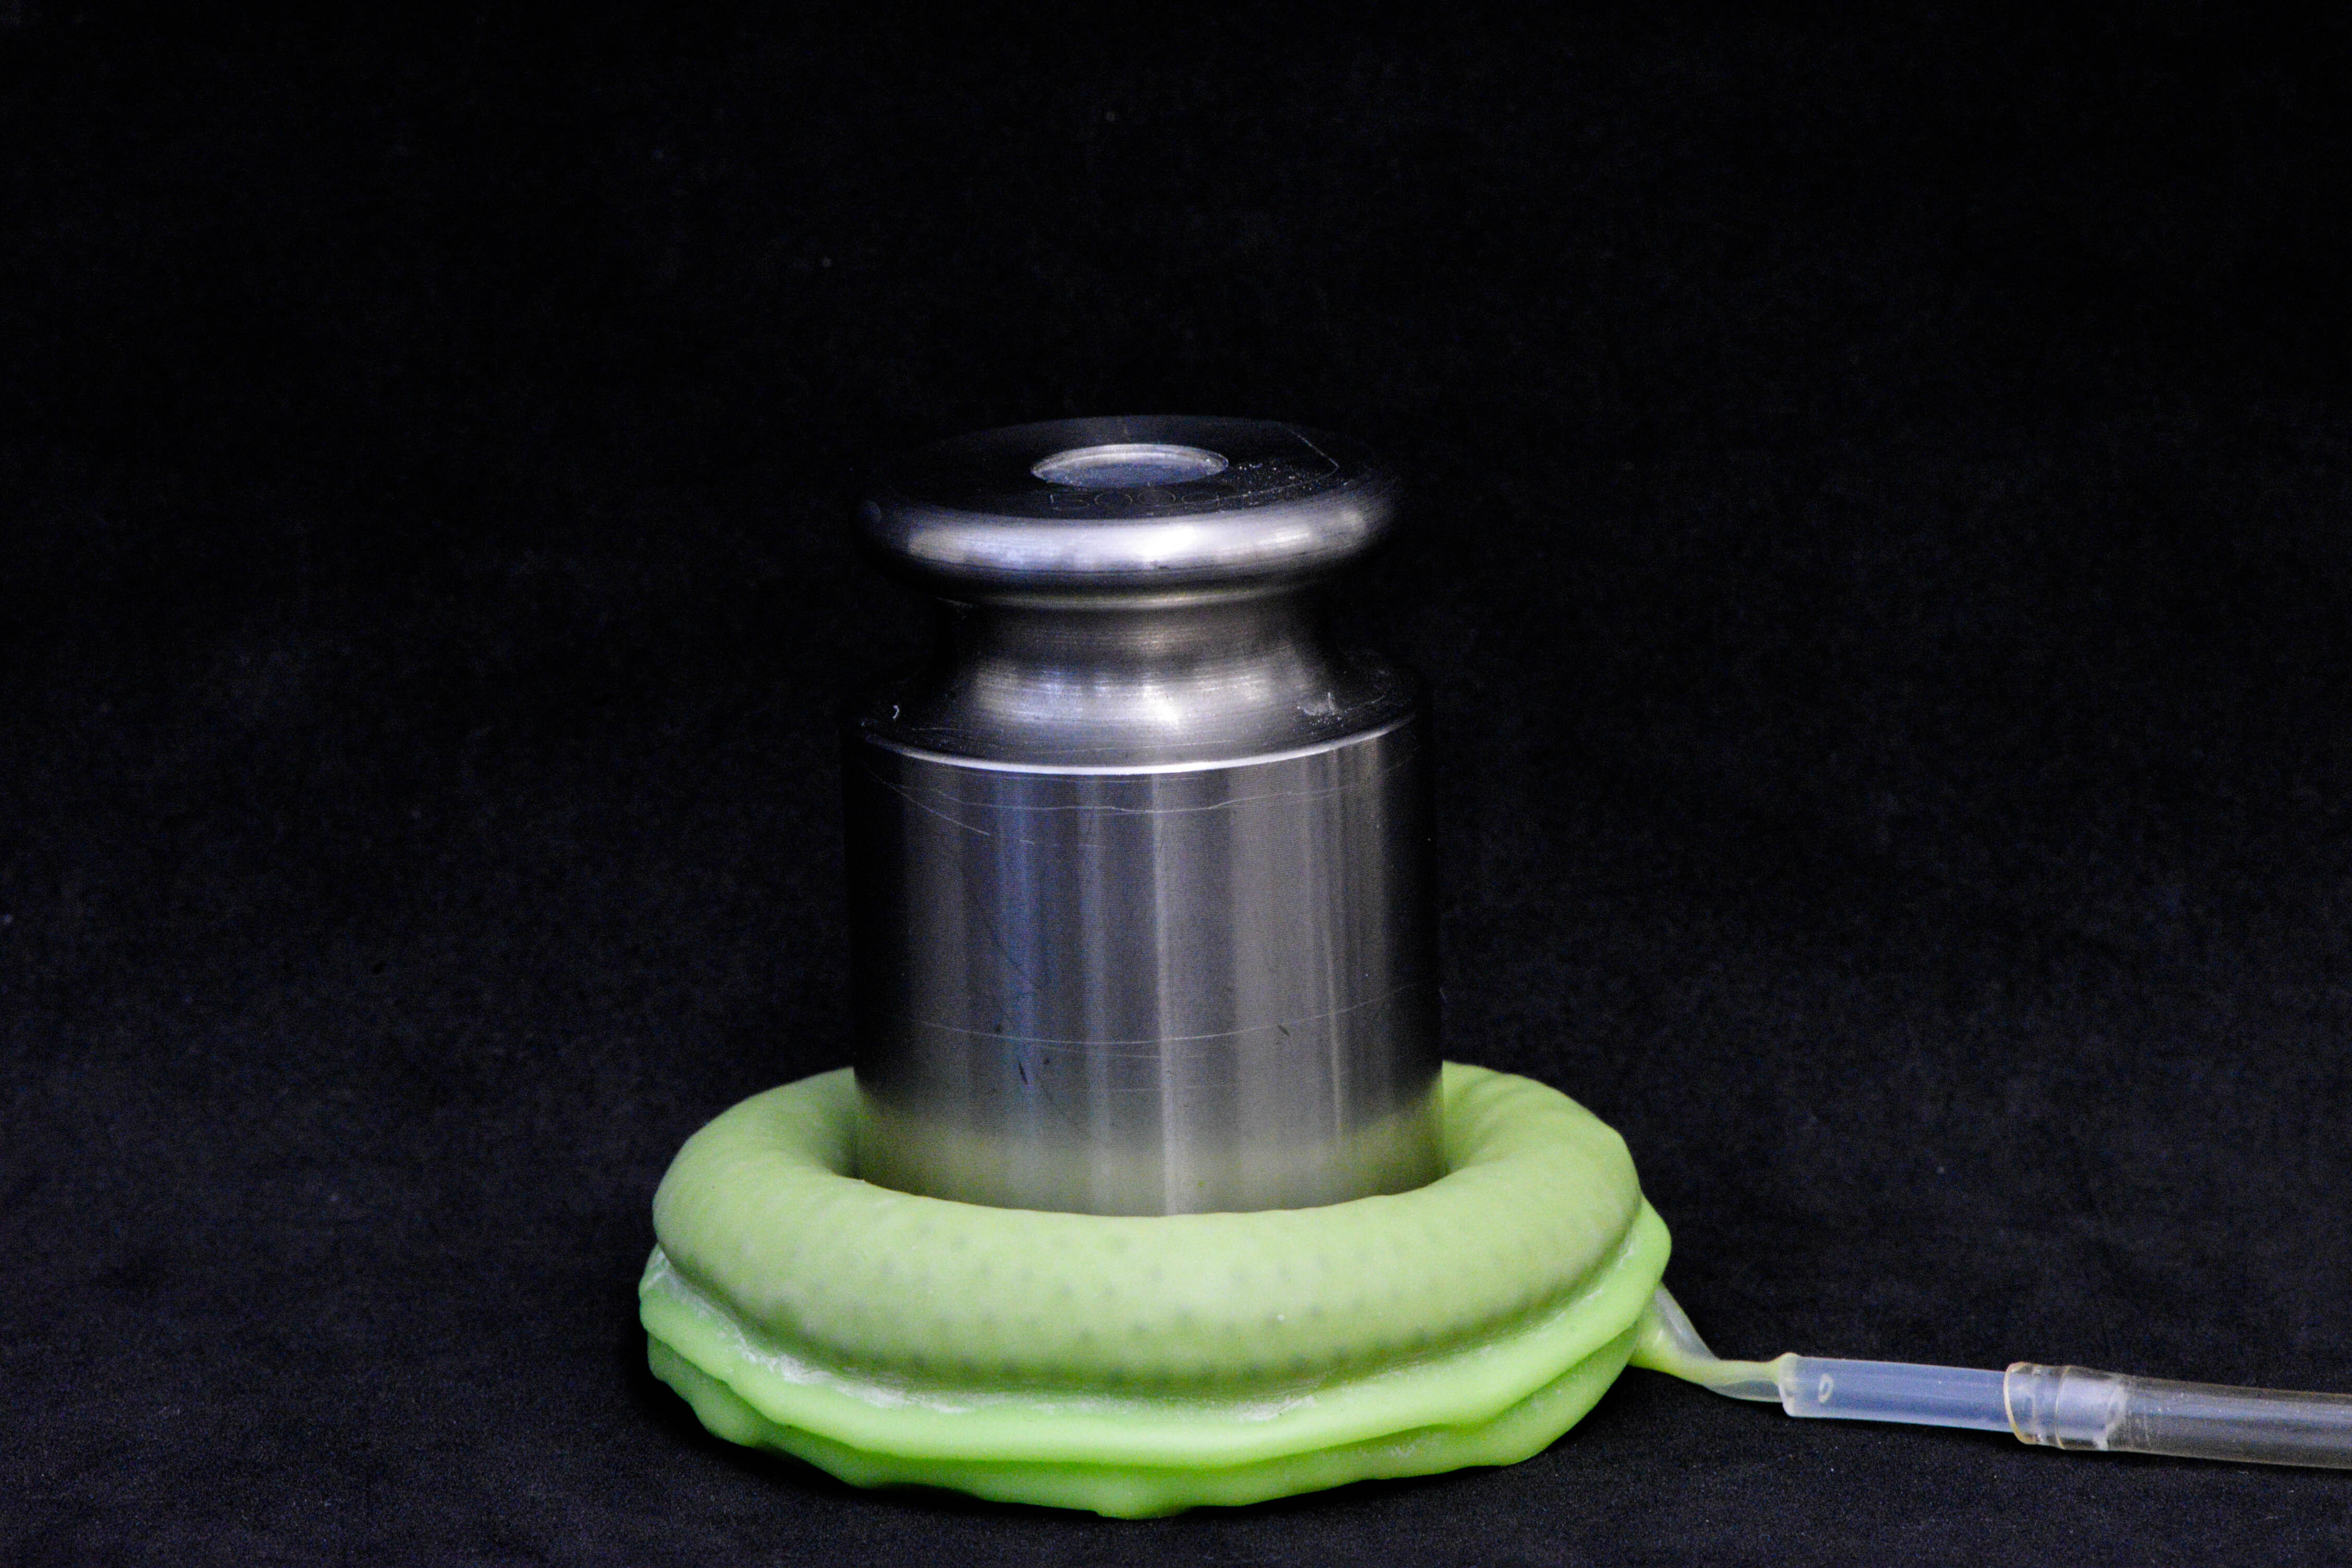
\includegraphics[height=1.5cm]{newShellCrushed-2}};
	
	% Plot the right triangle
	\addplot[line join=bevel, mark=none, thick,black] coordinates {(-.05,-.05) (-.05,2.6) (3.188,2.6) (-.05,-.05)};	
	\addplot[line join=bevel, mark=none, thick,black] coordinates {(-.08,-.05) (3.188,-.05) (3.188,1.275) (-.07,-.05)};
	
	% Annotate the triangle sides
	\node at (axis cs:1.45,3.3) [black]{$k$};
	\node at (axis cs:3.95,0.625) [black]{$k_o$};
	
	% Plot F_c
	\addplot[domain=0:10.38, dashed, black] {11.53};
	
	% Plot del_c
	\addplot[domain=0:11.53, samples=2, dashed, black] ({10.38}, {x});
	
	\addlegendentry[scale=0.75]{25 kPa}
	\addlegendentry[scale=0.75]{0 kPa}
	\addlegendentry[scale=0.75]{empty}
	

\end{axis}	

\end{tikzpicture}

\end{document}